\newpage
\section{Resultados}

Os resultados obtidos foram os seguintes.

\subsection{Resultados para tensão de entrada a 30V}

A tabela \ref{t_n30v} mostra os dados obtidos durante o experimento e a figura \ref{f_n30v} mostra o gráfico da eficiência para o conversor.

\begin{small}
	\begin{table}[H]
		\begin{center}
			\caption{Rendimento para tensão de entrada 30V e tensão de saída 15V}
			\begin{tabular}{l|l|l|l|l}
				\hline
				Tensão de & Corrente de & Tensão de  & Corrente de & Rendimento\\
				entrada [V]& entrada [A] & saída [V] & saída [A] &\\
				\hline
				30.0 & 0.22 & 15.0 & 0.251  & 0.6705\\
				\hline
				30.0 & 0.30 & 15.0 & 0.504  & 0.8400\\
				\hline
				30.0 & 0.44 & 15.0 & 0.758  & 0.8614\\
				\hline
				30.0 & 0.56 & 15.0 & 1.002  & 0.8946\\
				\hline
				30.0 & 0.69 & 15.0 & 1.249  & 0.9051\\
				\hline
				30.0 & 0.82 & 15.0 & 1.510 & 0.9207\\
				\hline
				30.0 & 0.98 & 15.0 & 1.749 & 0.8923\\
				\hline
				30.0 & 1.07 & 15.0 & 2.001  & 0.9350\\
				\hline
				30.0 & 1.17 & 15.0 & 2.249  & 0.9611\\
				\hline
				30.0 & 1.30 & 15.0 & 2.508  & 0.9646\\
				\hline
				30.0 & 1.48 & 15.0 & 2.751 & 0.9294\\
				\hline
				30.0 & 1.62 & 15.0 & 3.010 & 0.9290\\
				\hline
			\end{tabular}
			\label{t_n30v}
		\end{center}
	\end{table}
\end{small}

\begin{figure}[H]
	\centering
	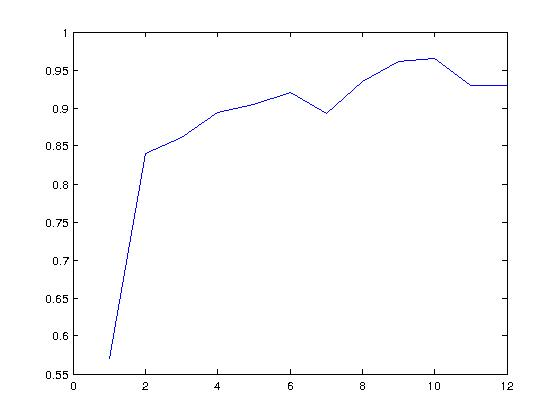
\includegraphics[scale=0.5]{Imagens/n30v.jpg}
	\caption{Eficiência do conversor buck para $V_e$ de 30V.}
	\label{f_n30v}
\end{figure}

\subsection{Resultados para tensão de entrada a 30V}

A tabela \ref{t_n20v} mostra os dados obtidos durante o experimento e a figura \ref{f_n20v} mostra o gráfico da eficiência para o conversor.

\begin{small}
	\begin{table}[H]
		\begin{center}
			\caption{Rendimento para tensão de entrada 20V e tensão de saída 15V}
			\begin{tabular}{l|l|l|l|l}
				\hline
				Tensão de & Corrente de & Tensão de  & Corrente de & Rendimento\\
				entrada [V]& entrada [A] & saída [V] & saída [A] &\\
				\hline
				20.0 & 0.198 & 15.0 & 0.250  & 0.6313\\
				\hline
				20.0 & 0.301 & 15.0 & 0.501  & 0.8322\\
				\hline
				20.0 & 0.45 & 15.0 & 0.749  & 0.8322\\
				\hline
				20.0 & 0.56 & 15.0 & 1.000  & 0.8929\\
				\hline
				20.0 & 0.69 & 15.0 & 1.250  & 0.9058\\
				\hline
				20.0 & 0.82 & 15.0 & 1.501 & 0.9381\\
				\hline
				20.0 & 0.97 & 15.0 & 1.750 & 0.9021\\
				\hline
				20.0 & 1.10 & 15.0 & 1.998  & 0.9082\\
				\hline
				20.0 & 1.22 & 15.0 & 2.251  & 0.9225\\
				\hline
				20.0 & 1.31 & 15.0 & 2.500  & 0.9542\\
				\hline
				20.0 & 1.43 & 15.0 & 2.749 & 0.9612\\
				\hline
				20.0 & 1.62 & 15.0 & 3.000 & 0.9259\\
				\hline
			\end{tabular}
			\label{t_n20v}
		\end{center}
	\end{table}
\end{small}

\begin{figure}[H]
	\centering
	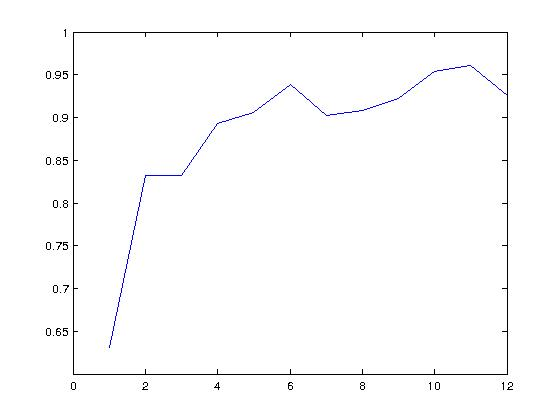
\includegraphics[scale=0.5]{Imagens/n20v.jpg}
	\caption{Eficiência do conversor buck para $V_e$ de 20V.}
	\label{f_n20v}
\end{figure}

\subsection{Tensão de chaveamento}
A figura \ref{f_vch} mostra a forma de onda da tensão na chave do conversor. A imagem foi obtida com o osciloscópio.

\begin{figure}[H]
	\centering
	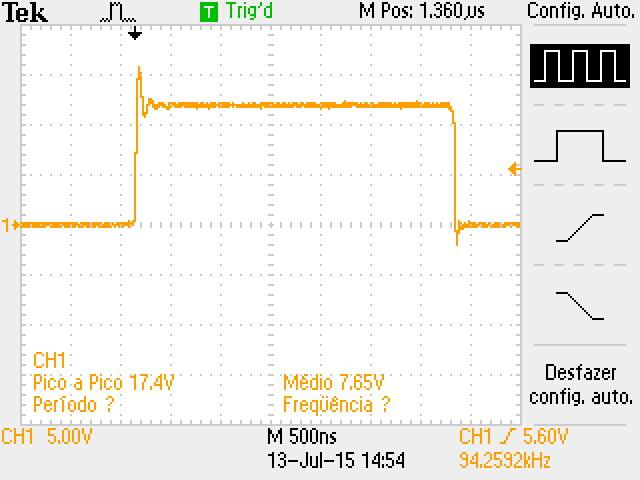
\includegraphics[scale=0.5]{Imagens/Vch.jpg}
	\caption{Forma de onda na chave do conversor.}
	\label{f_vch}
\end{figure}